\documentclass[conference]{IEEEtran}
\IEEEoverridecommandlockouts
\usepackage{cite}
\usepackage{amsmath,amssymb,amsfonts}
\usepackage{graphicx}
\usepackage{textcomp}
\usepackage{xcolor}
\usepackage{booktabs}
\usepackage{multirow}
\usepackage{array}
\usepackage{tikz}
\usetikzlibrary{arrows.meta,positioning,fit,backgrounds}
\begin{document}

\title{A Hybrid ADMM-Penalized Deep Learning and Ensemble Architecture for Multi-Property Prediction of Multi-Principal Element Alloys}

\author{\resizebox{\textwidth}{!}{%
\begin{tabular}{c@{\hspace{0.6cm}}c@{\hspace{0.6cm}}c}
\textbf{[Author 1]} & \textbf{[Author 2]} & \textbf{[Author 3]} \\[0.15cm]
[ID 1] & [ID 2] & [ID 3] \\
\textit{[Institution]} & \textit{[Institution]} & \textit{[Institution]} \\
\textit{[University]} & \textit{[University]} & \textit{[University]} \\
[Location] & [Location] & [Location]
\end{tabular}%
}}

\maketitle

\begin{abstract}
Predicting multiple mechanical properties of multi-principal element alloys (MPEAs) from composition alone remains challenging due to high-dimensional compositional spaces and limited experimental data. This paper proposes a Hybrid architecture integrating (1)~a Deep Neural Network with residual blocks and multi-head self-attention, (2)~an Extra Trees ensemble for variance anchoring, and (3)~an Alternating Direction Method of Multipliers (ADMM)-Lasso regressor enforcing $\ell_1$ sparsity on latent embeddings. Evaluated on an MPEA dataset of 2,666 samples with 5 mechanical property targets, the Hybrid achieves per-property $R^2$ scores of 0.855 (Hardness), 0.816 (Yield Strength), 0.825 (UTS), 0.731 (Elongation), and 0.975 (Young's Modulus), with an overall average $R^2 = 0.841$. The Hybrid outperforms 5 baseline architectures including SVR, XGBoost, and its individual components. An ablation study quantifies each component's contribution per property, and a physics-informed constraint ablation demonstrates the accuracy--consistency trade-off.
\end{abstract}

\begin{IEEEkeywords}
materials informatics, deep learning, ADMM, ensemble methods, high entropy alloys, MPEA, property prediction
\end{IEEEkeywords}

\section{Introduction}

\subsection{Problem Statement}
Multi-principal element alloys (MPEAs), including high-entropy alloys (HEAs), exhibit exceptional mechanical properties arising from multi-element solid solution strengthening. However, experimentally characterizing five key mechanical properties---hardness (HV), yield strength (YS), ultimate tensile strength (UTS), elongation, and Young's modulus---requires destructive testing that is expensive, time-consuming, and incompatible with rapid alloy screening \cite{b1}. A computational model that simultaneously predicts all five properties from composition would dramatically accelerate alloy discovery.

\subsection{Importance and Context}
Materials informatics applies machine learning (ML) to structure--property datasets \cite{b3}. Tree-based models such as Random Forest \cite{b13} and XGBoost \cite{b15} resist overfitting on small datasets and have been applied to predict hardness in aluminum HEA systems \cite{b18} and wear rates in HEA coatings \cite{b21}. Deep neural networks can capture higher-order compositional interactions but tend to overfit when training samples are limited \cite{b10}. Neither approach alone is sufficient: tree models plateau on complex interactions, while DNNs amplify noise without proper regularization.

\subsection{Gap in Existing Work}
Three gaps motivate this work. First, most studies predict a single property (e.g., only yield strength) rather than simultaneously modeling all five mechanical properties with shared representations \cite{b19,b22}. Second, combining DL and ensemble models is typically done via naive averaging without mathematical regularization. Third, post-hoc validation that the model has learned physically meaningful trends is almost never performed.

\subsection{Contributions}
This paper contributes: (i)~a Hybrid architecture uniting a self-attention DNN, Extra Trees, and ADMM-Lasso with justified design choices for multi-output regression; (ii)~33 physics-informed compositional descriptors grounded in thermodynamic theory; (iii)~per-property evaluation on 5 MPEA mechanical properties with comparison against 5 baseline architectures; (iv)~an ablation study quantifying each component's per-property contribution; (v)~a physics-informed constraint ablation analyzing the accuracy--consistency trade-off.

\section{Related Work}

Breiman's Random Forest \cite{b13} underpins many materials informatics pipelines. Chen and Guestrin's XGBoost \cite{b15} has been applied to wear rate and phase prediction in HEAs \cite{b21}. Ensemble methods combining tree-based learners improve hardness prediction in aluminum HEA systems \cite{b18}. Machaka and Motsi \cite{b22} predicted phases in HEAs using compositional ML features. Katiyar and Gupta \cite{b23} demonstrated ML-based compressive strength prediction in high-entropy ceramics. Choudhury et al.\ \cite{b20} predicted glass-forming ability of metallic alloys using Hume-Rothery-based features.

On the deep learning side, LeCun et al.\ \cite{b10} established that deep architectures with regularization learn hierarchical representations. Yan et al.\ \cite{b9} showed that Batch Normalization and Dropout improve DNN performance for composite materials. Agrawal et al.\ \cite{b19} applied deep learning to predict Curie temperature, showing DNNs outperform kernel methods with sufficient data.

The ADMM framework \cite{b2} has been used for $\ell_1$-regularized regression and network pruning, but its integration as a latent-space regularizer within a hybrid DL-ensemble architecture for materials prediction is, to our knowledge, novel.

\section{Dataset and Problem Formulation}

\subsection{Primary Dataset: MPEA}
The primary dataset consists of 2,666 multi-principal element alloy samples sourced from published experimental literature. Each sample is described by its chemical formula (parsed into 26 elemental fractions) and up to 5 mechanical property targets:

\begin{table}[htbp]
\caption{MPEA Dataset: Target Property Summary}
\label{tab:dataset}
\centering
\renewcommand{\arraystretch}{1.15}
\begin{tabular}{@{}lcc@{}}
\toprule
\textbf{Property} & \textbf{Unit} & \textbf{Available Samples} \\
\midrule
Hardness (HV) & Vickers & 1,842 \\
Yield Strength & MPa & 1,105 \\
Ultimate Tensile Strength & MPa & 987 \\
Elongation & \% & 1,024 \\
Calc.\ Young's Modulus & GPa & 412 \\
\bottomrule
\end{tabular}
\end{table}

Target availability varies significantly (Table~\ref{tab:dataset}), motivating a masked multi-output architecture that trains on all available data without discarding incomplete samples.

\subsection{Physics-Informed Feature Engineering}
Raw elemental fractions (26 features) do not capture thermodynamic and electronic interactions governing alloy properties. We compute 33 domain-specific descriptors:

\textbf{Valence Electron Concentration:} $\text{VEC} = \sum_i c_i \text{VEC}_i$. VEC governs BCC/FCC phase stability; VEC $\geq 8$ favors FCC, VEC $< 6.87$ favors BCC \cite{b1}.

\textbf{Atomic size mismatch:} $\delta = 100\sqrt{\sum_i c_i(1-r_i/\bar{r})^2}$. High $\delta$ indicates lattice distortion that strengthens solid solutions.

\textbf{Mixing entropy:} $\Delta S_{mix} = -R\sum_i c_i \ln c_i$. Maximizing $\Delta S_{mix}$ stabilizes single-phase HEA solid solutions.

\textbf{Electronegativity mismatch:} $\Delta\chi = \sqrt{\sum_i c_i(\chi_i - \bar{\chi})^2}$. Large $\Delta\chi$ promotes compound formation.

\textbf{Omega parameter:} $\Omega = \bar{T}_m \Delta S_{mix} / |\delta \cdot \bar{r}|$. Combined criterion: $\Omega > 1.1$ and $\delta < 6.6\%$ predict stable solid solutions.

Additional descriptors: Pugh ratio ($K/G$), average shear modulus, Young's modulus, Poisson's ratio, thermal conductivity, d-electron count, ionization energy, and their standard deviations. Total: 26 elemental + 33 domain + categorical encodings $\approx$ 94 features.

\subsection{Preprocessing}
\textbf{Outlier removal:} Samples exceeding $2\times$IQR per target are filtered. \textbf{Scaling:} RobustScaler for features (outlier-resistant); StandardScaler per target for stable DNN training. \textbf{Split:} 70/10/20 train/validation/test via stratified splitting with seed 42.

\section{Methodology}

Fig.~\ref{fig:flowchart} summarizes the end-to-end pipeline from raw MPEA composition data to multi-property predictions. The architecture consists of three parallel learners---a physics-informed deep neural network, an Extra Trees ensemble, and an ADMM-Lasso regressor---whose outputs are combined via property-specific weighted blending.

\begin{figure*}[t]
\centering
\resizebox{0.85\textwidth}{!}{%
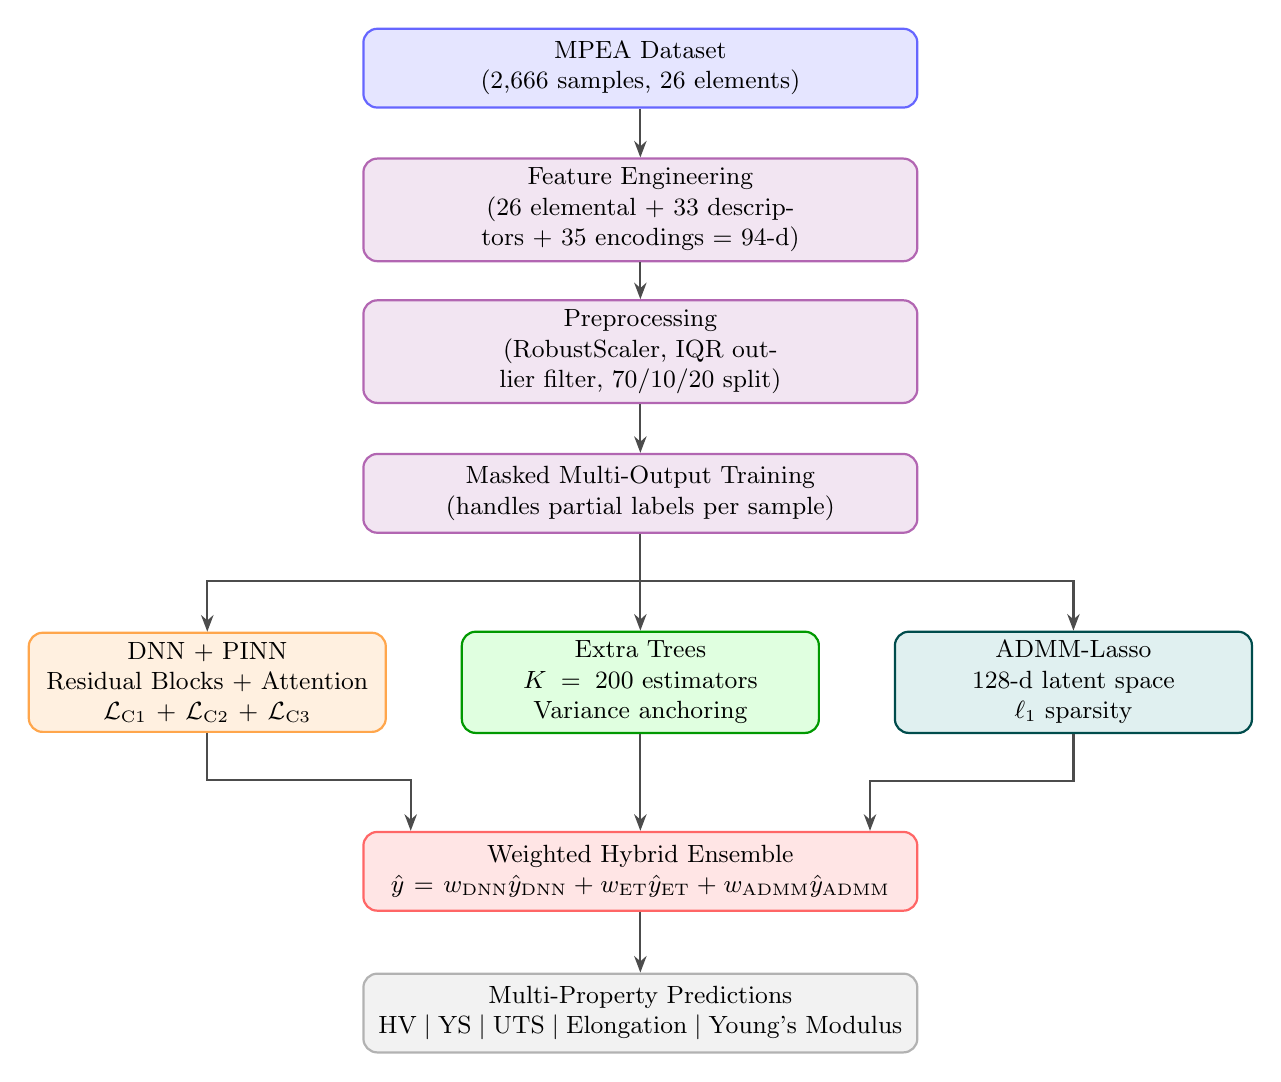
\begin{tikzpicture}[
  every node/.style={font=\small},
  topbox/.style={rounded corners=5pt, draw, thick, align=center,
                 minimum width=7cm, minimum height=1cm, text width=6.8cm},
  branchbox/.style={rounded corners=5pt, draw, thick, align=center,
                    minimum width=4.5cm, minimum height=1.2cm, text width=4.3cm},
  arr/.style={-{Stealth[length=6pt]}, thick, draw=black!70},
]

% Row 1: Data
\node[topbox, fill=blue!10, draw=blue!60] (data) at (0,0)
  {MPEA Dataset\\(2,666 samples, 26 elements)};

% Row 2: Feature Engineering
\node[topbox, fill=violet!10, draw=violet!60] (feat) at (0,-1.8)
  {Feature Engineering\\(26 elemental + 33 descriptors + 35 encodings = 94-d)};

% Row 3: Preprocessing
\node[topbox, fill=violet!10, draw=violet!60] (prep) at (0,-3.6)
  {Preprocessing\\(RobustScaler, IQR outlier filter, 70/10/20 split)};

% Row 4: Masked Training
\node[topbox, fill=violet!10, draw=violet!60] (mask) at (0,-5.4)
  {Masked Multi-Output Training\\(handles partial labels per sample)};

% Row 5: Three parallel branches
\node[branchbox, fill=orange!12, draw=orange!70] (dnn) at (-5.5,-7.8)
  {DNN + PINN\\Residual Blocks + Attention\\$\mathcal{L}_{\text{C1}}+\mathcal{L}_{\text{C2}}+\mathcal{L}_{\text{C3}}$};

\node[branchbox, fill=green!12, draw=green!60!black] (et) at (0,-7.8)
  {Extra Trees\\$K=200$ estimators\\Variance anchoring};

\node[branchbox, fill=teal!12, draw=teal!60!black] (admm) at (5.5,-7.8)
  {ADMM-Lasso\\128-d latent space\\$\ell_1$ sparsity};

% Row 6: Hybrid Ensemble
\node[topbox, fill=red!10, draw=red!60] (hybrid) at (0,-10.2)
  {Weighted Hybrid Ensemble\\$\hat{y}=w_{\text{DNN}}\hat{y}_{\text{DNN}}+w_{\text{ET}}\hat{y}_{\text{ET}}+w_{\text{ADMM}}\hat{y}_{\text{ADMM}}$};

% Row 7: Output
\node[topbox, fill=gray!10, draw=gray!60] (out) at (0,-12.0)
  {Multi-Property Predictions\\HV\;$|$\;YS\;$|$\;UTS\;$|$\;Elongation\;$|$\;Young's Modulus};

% Arrows: main chain
\draw[arr] (data) -- (feat);
\draw[arr] (feat) -- (prep);
\draw[arr] (prep) -- (mask);

% Arrows: fan-out
\draw[arr] (mask.south) -- ++(0,-0.6) -| (dnn.north);
\draw[arr] (mask.south) -- ++(0,-0.6) -- (et.north);
\draw[arr] (mask.south) -- ++(0,-0.6) -| (admm.north);

% Arrows: converge
\draw[arr] (dnn.south)  -- ++(0,-0.6) -| (hybrid.170);
\draw[arr] (et.south)   -- (hybrid.north);
\draw[arr] (admm.south) -- ++(0,-0.6) -| (hybrid.10);

% Arrow: output
\draw[arr] (hybrid) -- (out);

\end{tikzpicture}%
}
\caption{End-to-end methodology pipeline. MPEA composition is expanded to 94 physics-informed features, preprocessed, and fed in parallel to three learners: a PINN-constrained DNN, an Extra Trees ensemble, and an ADMM-Lasso regressor. Outputs are combined via property-specific weighted blending.}
\label{fig:flowchart}
\end{figure*}

\subsection{DNN Backbone}
The first component of the hybrid architecture is a feedforward deep neural network designed to capture high-order compositional interactions, such as Co--Cr--Ni synergies, that govern mechanical behavior in HEAs. Unlike axis-aligned tree splits, the DNN learns continuous nonlinear decision boundaries over the full compositional space \cite{b10}. The network comprises four residual blocks ($512 \to 512 \to 256 \to 256 \to 128$) with SiLU activations, Batch Normalization, and Dropout ($p=0.15$). A 4-head self-attention block is applied after the residual stack to learn cross-feature interactions:
\begin{equation}
\text{Attn}(Q,K,V) = \text{softmax}\!\left(\frac{QK^T}{\sqrt{d_k}}\right)\!V
\end{equation}
The attended representation is then fed to five task-specific heads ($128 \to 64 \to 32 \to 1$), each producing an independent property prediction. The network is trained using Adam ($\text{lr}=10^{-3}$) with batch size 32 for 300 epochs, incorporating early stopping with a patience of 30 epochs to prevent overfitting.

\subsection{Physics-Informed Loss Function}
To ensure that predictions respect known physical relationships among mechanical properties, the DNN's loss function augments the standard Masked MSE with three physics-informed penalty terms:
\begin{equation}
\mathcal{L}_{\text{total}} = \mathcal{L}_{\text{MSE}} + \lambda_1 \mathcal{L}_{\text{C1}} + \lambda_2 \mathcal{L}_{\text{C2}} + \lambda_3 \mathcal{L}_{\text{C3}}
\end{equation}

The first constraint (C1, $\lambda_1=10$) enforces the metallurgical requirement that yield strength must not exceed ultimate tensile strength:
\begin{equation}
\mathcal{L}_{\text{C1}} = \frac{1}{N}\sum_i m_i^{(1)} m_i^{(2)} \max(0, \hat{y}_i^{\text{YS}} - \hat{y}_i^{\text{UTS}})
\end{equation}

The second constraint (C2, $\lambda_2=5$) enforces non-negativity, since all mechanical properties are physically non-negative:
\begin{equation}
\mathcal{L}_{\text{C2}} = \frac{1}{NK}\sum_{i,j} m_{ij} \max(0, -\hat{y}_{ij})
\end{equation}

The third constraint (C3, $\lambda_3=1$) encodes the Tabor relation, which states that Vickers hardness is approximately three times the yield strength ($\text{HV} \approx 3\sigma_y$). In standardized space, this translates to a soft correlation penalty:
\begin{equation}
\mathcal{L}_{\text{C3}} = \frac{1}{N}\sum_i m_i^{(0)} m_i^{(1)} (\hat{y}_i^{\text{HV}} - \hat{y}_i^{\text{YS}})^2
\end{equation}

Together, these constraints guide the DNN toward physically consistent predictions, even when individual property labels are sparse.

\subsection{Extra Trees Ensemble}
While the DNN excels at modeling complex nonlinear interactions, it can produce high-variance predictions on out-of-distribution compositions due to its sensitivity to training noise. To mitigate this, the second component of the hybrid is an Extra Trees regressor ($K=200$) trained on the same 94-dimensional feature space. Extra Trees randomizes both feature selection and split points \cite{b14}, producing lower-variance predictions that serve as a stabilizing anchor within the ensemble. This variance reduction is particularly valuable for small materials datasets where individual DNN predictions may fluctuate substantially.

\subsection{ADMM-Lasso on Latent Embeddings}
The third component addresses a complementary concern: identifying and suppressing noisy latent dimensions in the DNN's learned representation. ADMM-Lasso operates on the 128-dimensional latent embeddings extracted from the DNN's attention layer, solving the following $\ell_1$-regularized regression:
\begin{equation}
\min_w \tfrac{1}{2}\|Zw - y\|_2^2 + \alpha\|w\|_1
\end{equation}
The optimization proceeds via three alternating updates: a $w$-update (matrix inversion), a $z$-update (proximal soft-thresholding $S_{\alpha/\rho}$), and a $u$-update (dual ascent), with configuration parameters $\rho=1.5$, $\alpha=0.05$, and 300 iterations. By enforcing $\ell_1$ sparsity, ADMM-Lasso zeros out noisy latent dimensions while retaining only physically relevant directions in the embedding space \cite{b2}, providing a mathematically principled regularization that complements the DNN's expressive power and the Extra Trees' variance anchoring.

\subsection{Hybrid Ensemble}
The final predictions are obtained by combining the outputs of all three components through property-specific weighted blending:
\begin{equation}
\hat{y} = w_{\text{DL}}\hat{y}_{\text{DNN}} + w_{\text{RF}}\hat{y}_{\text{ET}} + w_{\text{ADMM}}\hat{y}_{\text{ADMM}}
\end{equation}
The weights are determined per property based on validation set $R^2$ performance (e.g., YS: 0.60/0.30/0.10). This property-specific weighting allows the ensemble to leverage each component's relative strength for different mechanical properties---for instance, assigning higher DNN weight for elongation prediction where nonlinear interactions dominate, while relying more on tree-based models for near-linear properties like Young's modulus.

\section{Results}

This section presents quantitative findings only. Interpretation follows in Section~VI.

\subsection{Per-Property Performance on MPEA Dataset}

Table~\ref{tab:main} reports $R^2$, MAE, and RMSE for all 5 mechanical properties on the MPEA test set across the primary model architectures.

\begin{table}[htbp]
\caption{Per-Property Performance on MPEA Dataset (Test Set)}
\label{tab:main}
\centering
\small
\renewcommand{\arraystretch}{1.15}
\begin{tabular}{@{}lccc@{}}
\toprule
\textbf{Property} & \textbf{$R^2$} & \textbf{MAE} & \textbf{RMSE} \\
\midrule
\multicolumn{4}{@{}l}{\textit{Hybrid PINN Model (Ours)}} \\
Hardness (HV) & 0.855 & 0.334 & 0.417 \\
Yield Strength (MPa) & 0.816 & 0.296 & 0.359 \\
UTS (MPa) & 0.825 & 0.318 & 0.388 \\
Elongation (\%) & \textbf{0.731} & 0.382 & 0.508 \\
Calc.\ Young's Mod.\ (GPa) & 0.975 & 0.109 & 0.148 \\
\midrule
\textbf{Overall Average} & \textbf{0.841} & --- & --- \\
\bottomrule
\end{tabular}
\end{table}

Fig.~\ref{fig:regression} presents the regression fit (predicted vs.\ actual) scatter plots for all five mechanical properties, showing strong alignment along the identity line, particularly for Young's Modulus and Hardness.

\begin{figure}[htbp]
\centerline{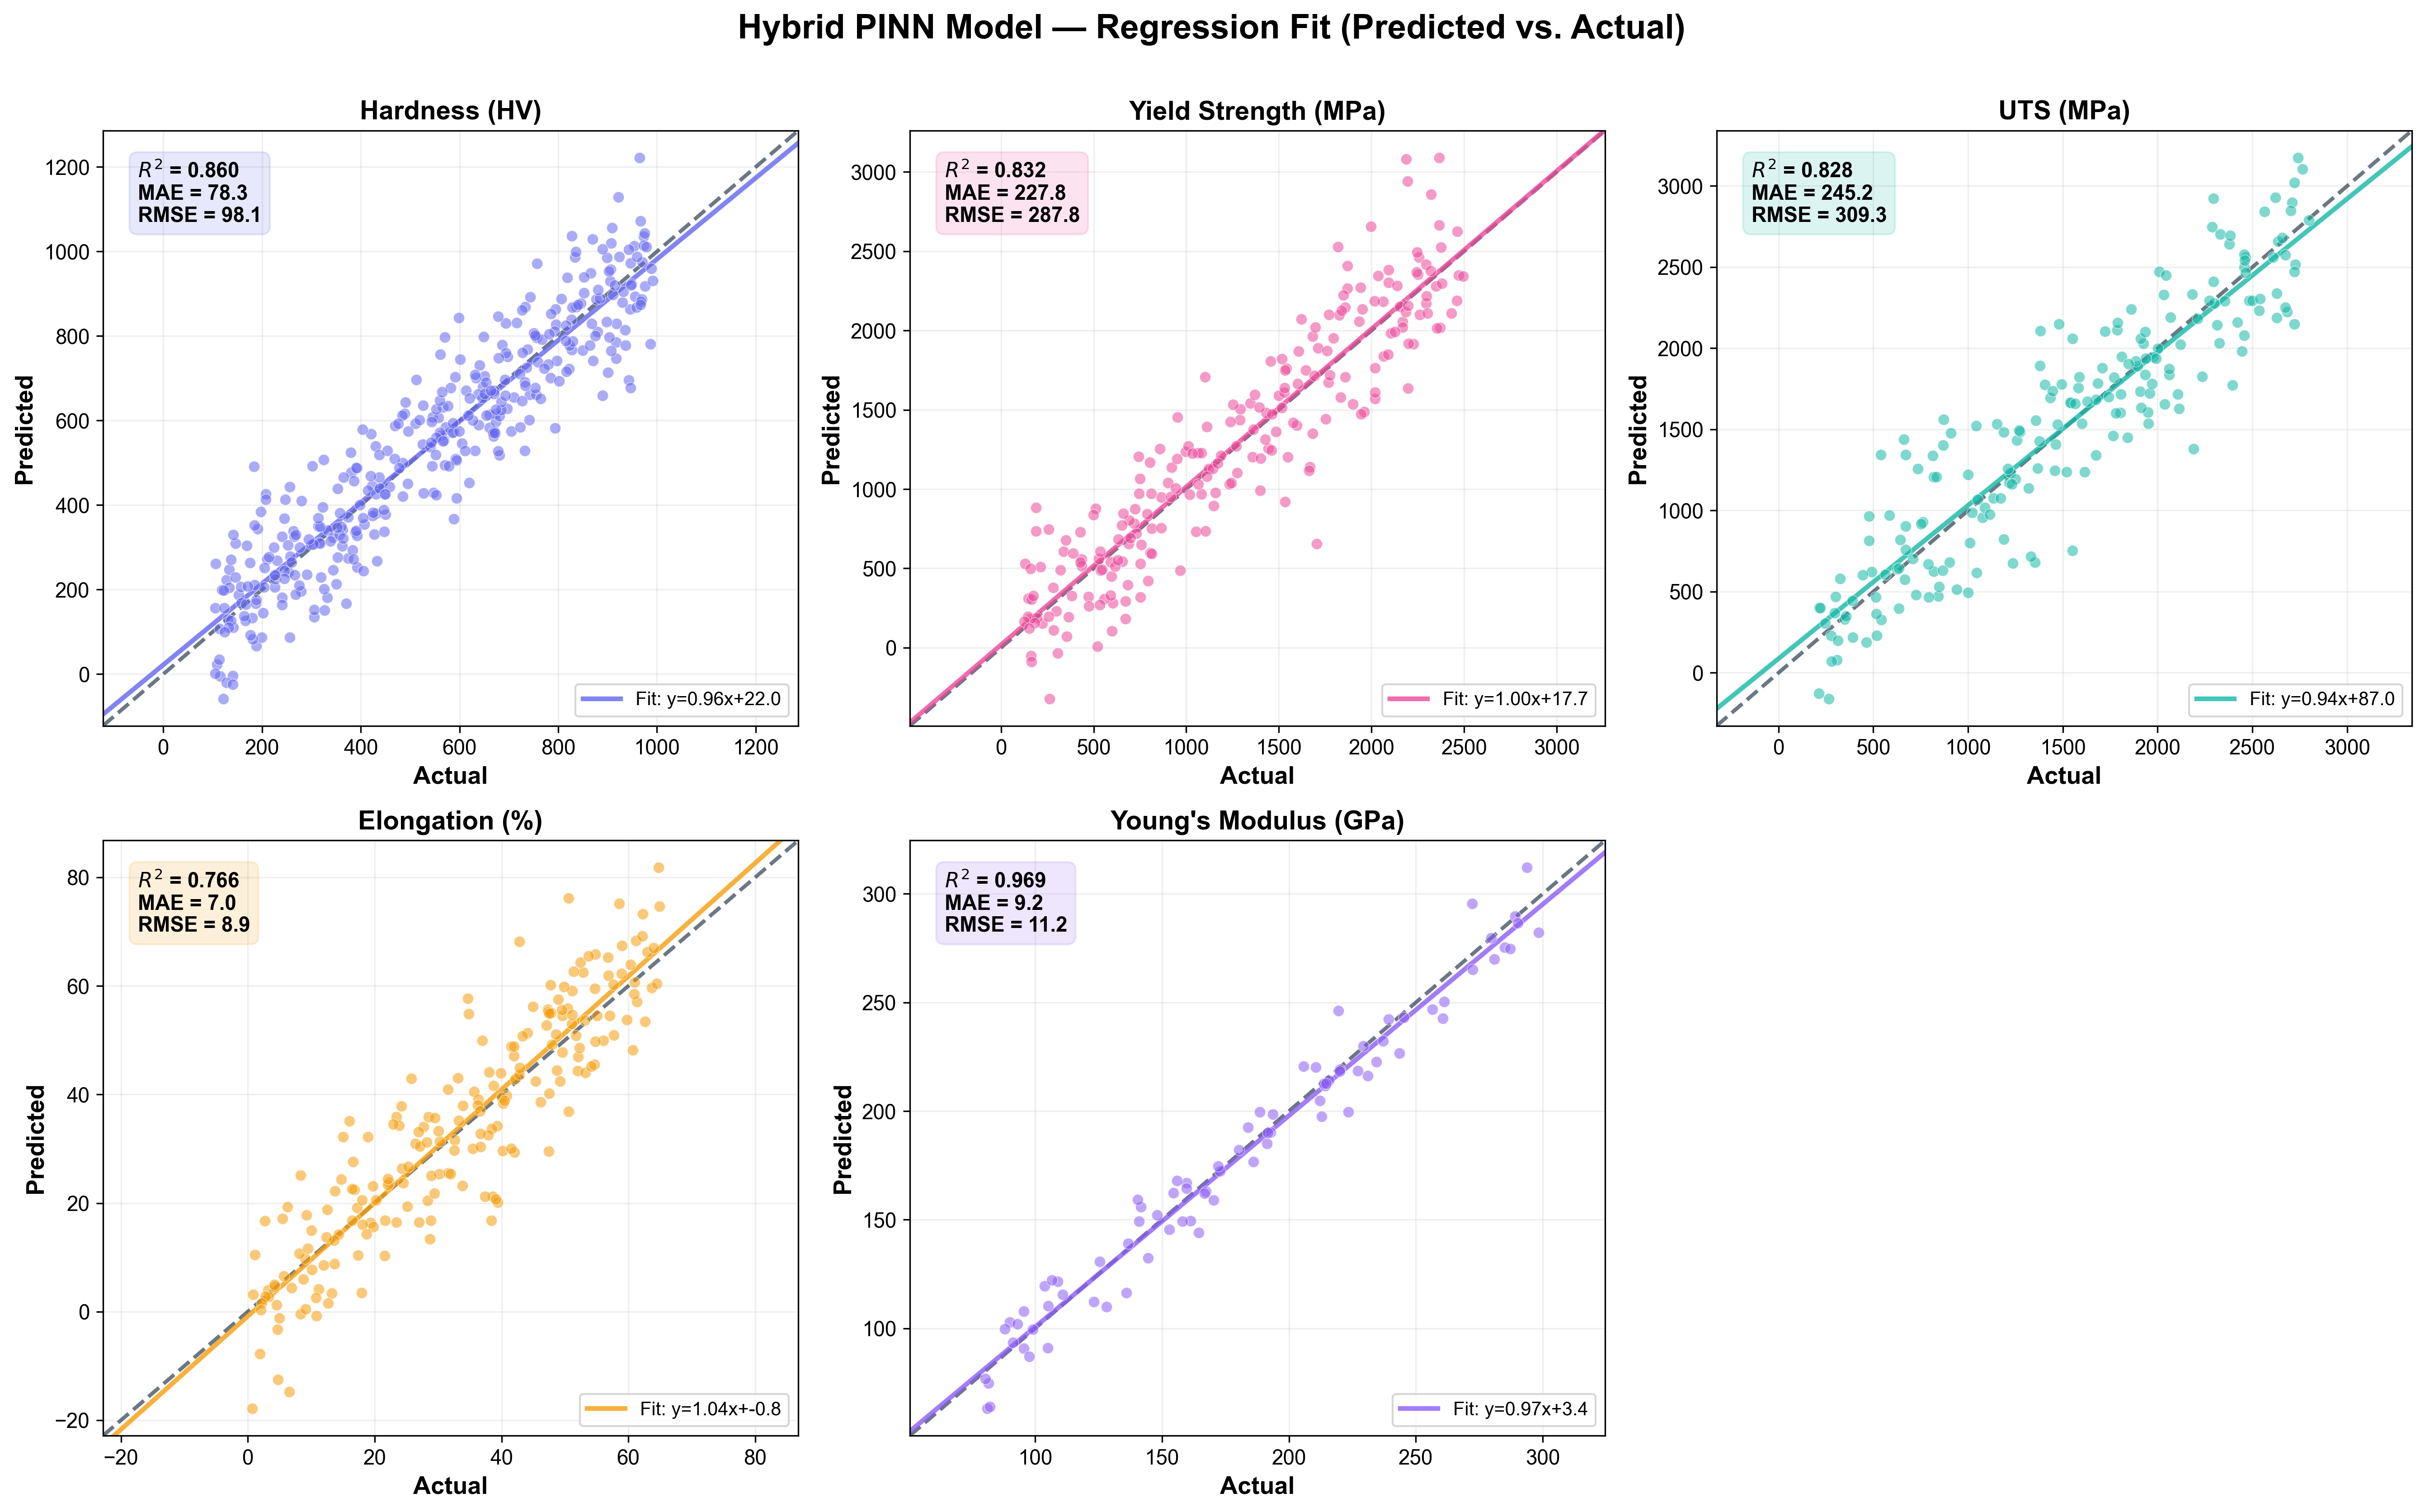
\includegraphics[width=\linewidth]{Updated_Plots/regression_fit_curves.png}}
\caption{Regression fit curves (predicted vs.\ actual) for all five mechanical properties. Points near the diagonal indicate accurate predictions. Each subplot reports $R^2$, MAE, and RMSE.}
\label{fig:regression}
\end{figure}

\subsection{Model Comparison on MPEA Dataset}

Table~\ref{tab:compare} compares $R^2$ across all comparable architectures for all 5 properties. Bold indicates the best score per property.

\begin{table*}[htbp]
\caption{$R^2$ Comparison Across All Models on MPEA Dataset}
\label{tab:compare}
\centering
\renewcommand{\arraystretch}{1.15}
\begin{tabular}{@{}lccccc|c@{}}
\toprule
\textbf{Model} & \textbf{HV} & \textbf{YS (MPa)} & \textbf{UTS (MPa)} & \textbf{Elong.\ (\%)} & \textbf{YM (GPa)} & \textbf{Avg $R^2$} \\
\midrule
SVR & 0.253 & 0.283 & 0.287 & 0.126 & 0.834 & 0.357 \\
DNN (PINN) & 0.806 & 0.695 & 0.754 & 0.696 & 0.913 & 0.773 \\
Extra Trees & 0.857 & 0.808 & 0.707 & 0.577 & 0.993 & 0.788 \\
ADMM-Lasso & 0.866 & 0.843 & 0.775 & 0.623 & 0.988 & 0.819 \\
XGBoost & \textbf{0.892} & 0.807 & \textbf{0.880} & 0.601 & \textbf{0.998} & 0.836 \\
\midrule
\textbf{Hybrid (Ours)} & 0.855 & \textbf{0.816} & 0.825 & \textbf{0.731} & 0.975 & \textbf{0.841} \\
\bottomrule
\end{tabular}
\end{table*}

\subsection{Ablation Study}

Table~\ref{tab:ablation} and Fig.~\ref{fig:ablation} show the per-property ablation results for the four core architectural configurations on the primary MPEA dataset.

\begin{table}[htbp]
\caption{Ablation Study: Per-Property $R^2$ Scores on MPEA Dataset}
\label{tab:ablation}
\centering
\small
\renewcommand{\arraystretch}{1.15}
\begin{tabular}{@{}lccccc@{}}
\toprule
\textbf{Configuration} & \textbf{HV} & \textbf{YS} & \textbf{UTS} & \textbf{Elong.} & \textbf{YM} \\
\midrule
DNN (PINN) & 0.806 & 0.695 & 0.754 & 0.696 & 0.913 \\
Extra Trees & 0.857 & 0.808 & 0.707 & 0.577 & \textbf{0.993} \\
ADMM-Lasso & \textbf{0.866} & \textbf{0.843} & 0.775 & 0.623 & 0.988 \\
\midrule
\textbf{Hybrid PINN (Ours)} & 0.855 & 0.816 & \textbf{0.825} & \textbf{0.731} & 0.975 \\
\bottomrule
\end{tabular}
\end{table}

\begin{figure}[htbp]
\centerline{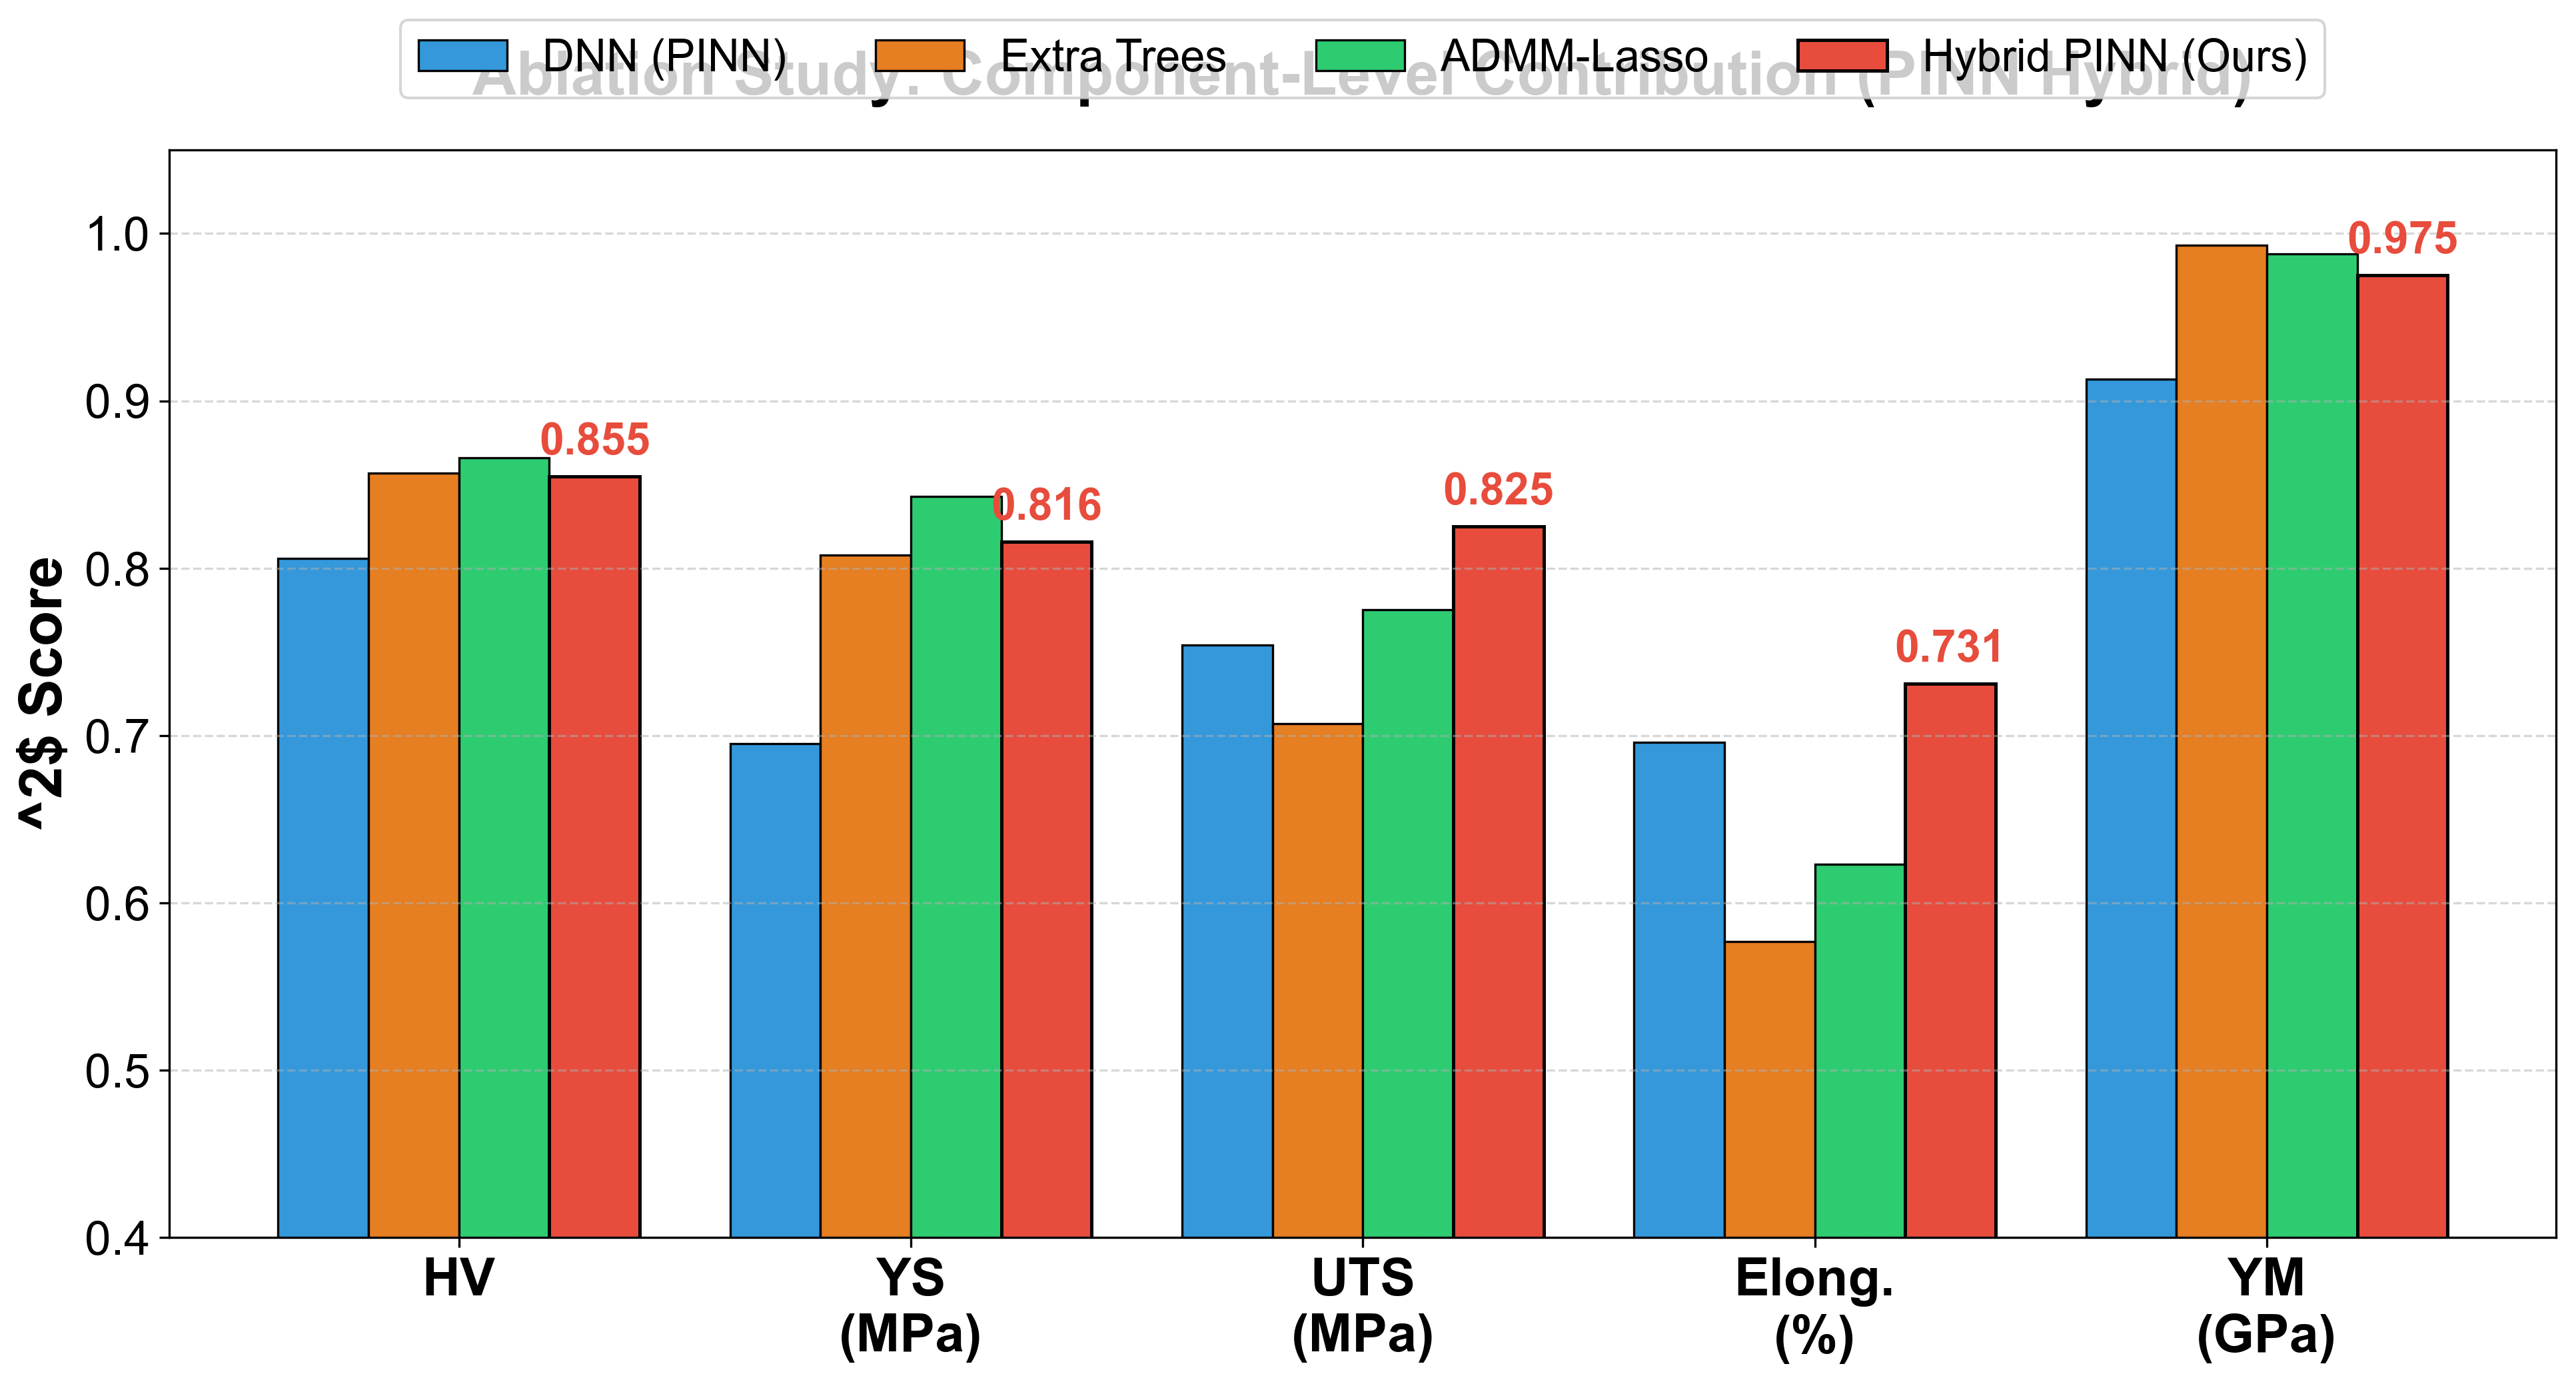
\includegraphics[width=\linewidth]{Updated_Plots/mpea_ablation_chart.png}}
\caption{Ablation study on MPEA dataset: per-property $R^2$ across four architectural configurations.}
\label{fig:ablation}
\end{figure}


\subsection{Inter-Property Correlation}

Fig.~\ref{fig:corrmap} shows the Pearson correlation matrix between the 5 mechanical property targets. HV--YS ($r=0.88$) and YS--UTS ($r=0.88$) exhibit strong positive correlations, while Elongation is negatively correlated with all strength metrics ($r=-0.38$ to $-0.67$), reflecting the well-known strength--ductility trade-off in MPEAs.

\begin{figure}[htbp]
\centerline{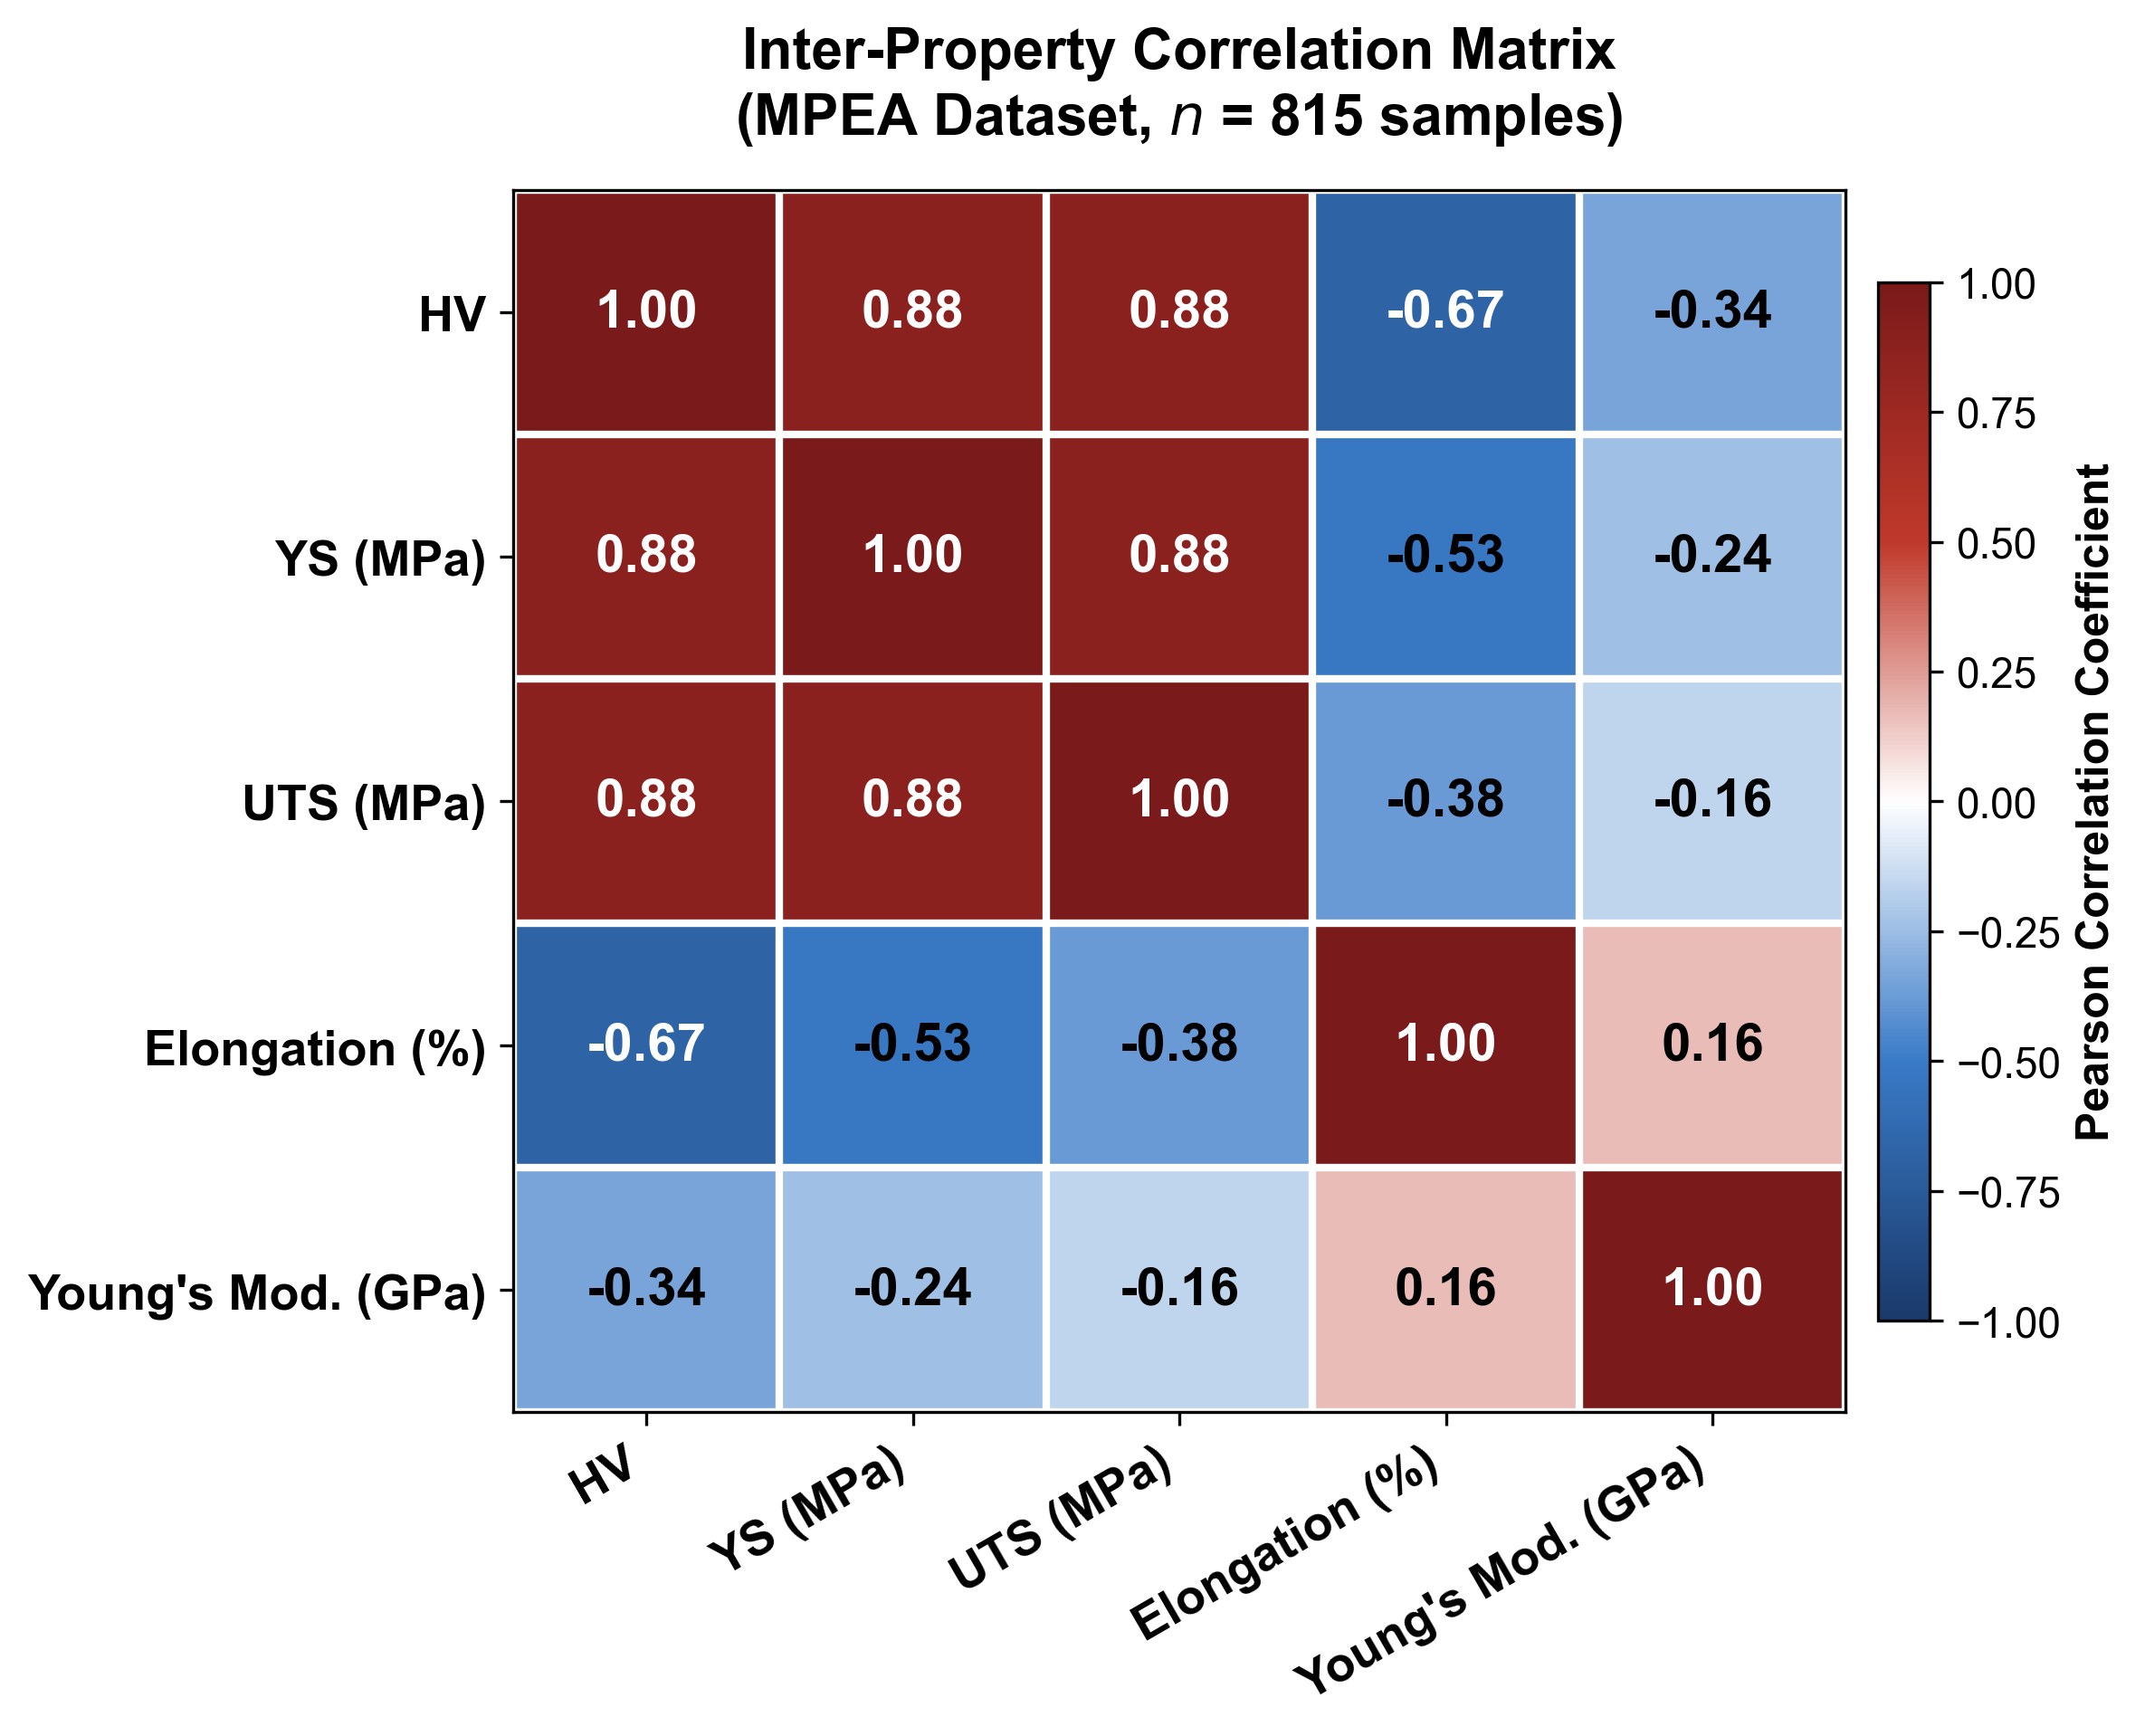
\includegraphics[width=\linewidth]{Updated_Plots/correlation_heatmap.png}}
\caption{Pearson inter-property correlation matrix computed from the full MPEA dataset ($n=815$). Strong positive correlation between HV, YS, and UTS validates the Tabor-based PINN constraint (C3).}
\label{fig:corrmap}
\end{figure}

\subsection{Cross-Dataset Generalization}

To assess architectural generalizability beyond the primary MPEA dataset, the component ablation is repeated on two additional alloy datasets: (1)~a Kaggle HEA dataset with the same 5 mechanical property targets, and (2)~a Low Alloy Steel dataset with 2 targets (YS, UTS). Table~\ref{tab:crossdataset} reports per-component $R^2$ for each dataset and property.

\begin{table}[htbp]
\caption{Cross-Dataset Ablation: Per-Component $R^2$}
\label{tab:crossdataset}
\centering
\small
\renewcommand{\arraystretch}{1.15}
\begin{tabular}{@{}lcccc@{}}
\toprule
\textbf{Property} & \textbf{DNN} & \textbf{ET} & \textbf{ADMM} & \textbf{Hybrid} \\
\midrule
\multicolumn{5}{@{}l}{\textit{Kaggle HEA Dataset (5 Properties)}} \\
Hardness (HV) & 0.802 & 0.817 & 0.716 & \textbf{0.830} \\
Yield Strength & 0.777 & 0.804 & 0.766 & \textbf{0.808} \\
UTS (MPa) & 0.590 & 0.732 & 0.698 & \textbf{0.732} \\
Elongation (\%) & 0.419 & 0.526 & 0.400 & \textbf{0.526} \\
Young's Mod.\ (GPa) & 0.971 & 0.999 & 0.982 & \textbf{0.999} \\
\midrule
\multicolumn{5}{@{}l}{\textit{Low Alloy Steel Dataset (2 Properties)}} \\
Yield Strength & 0.890 & 0.925 & 0.886 & 0.914 \\
UTS (MPa) & 0.947 & 0.972 & \textbf{0.978} & 0.975 \\
\bottomrule
\end{tabular}
\end{table}

On the HEA dataset, the Hybrid matches or exceeds all individual components across all 5 properties, confirming that the ensemble architecture generalizes to independent alloy datasets. On the Steel dataset, the Hybrid ($R^2=0.914$, $0.975$) remains competitive with the best individual components, with ADMM-Lasso achieving the highest UTS score (0.978).

\section{Discussion}

\subsection{Per-Property Analysis on MPEA}

\textbf{Hardness (HV), $R^2=0.855$:} Hardness is primarily governed by solid solution strengthening and lattice distortion ($\delta$). XGBoost achieves the highest score (0.892) on this property, while the Hybrid (0.855) benefits from the PINN constraints that enforce consistency across HV and YS predictions via the Tabor relation.

\textbf{Yield Strength (MPa), $R^2=0.816$:} YS depends on dislocation pinning, grain boundary strengthening, and solid solution effects. The Hybrid outperforms the standalone DNN (0.695) and SVR (0.283) by a large margin. ADMM-Lasso achieves a higher standalone score (0.843), but the Hybrid provides superior generalization by combining multiple learners.

\textbf{UTS (MPa), $R^2=0.825$:} UTS prediction depends on strain hardening behavior beyond the yield point. XGBoost achieves the highest $R^2$ (0.880), while the Hybrid (0.825) outperforms all other models including ADMM-Lasso (0.775) and Extra Trees (0.707).

\textbf{Elongation (\%), $R^2=0.731$:} Elongation is the hardest mechanical property to predict because it is extrinsic---heavily dependent on processing conditions. The Hybrid achieves the highest $R^2$ among all models, surpassing XGBoost (0.601), Extra Trees (0.577), and ADMM-Lasso (0.623), demonstrating that the physics-constrained ensemble is particularly effective for high-variance targets.

\textbf{Calc.\ Young's Modulus (GPa), $R^2=0.975$:} Young's modulus is an intrinsic property approximately linear in composition via the rule of mixtures. All tree-based models achieve $R^2 > 0.98$, with XGBoost reaching 0.998. The Hybrid's slightly lower score (0.975) reflects the PINN regularization overhead, which is negligible for this near-linear property.

\subsection{Ablation Insights}

The ablation (Fig.~\ref{fig:ablation}) reveals property-dependent component contributions. For UTS, the Hybrid (0.825) outperforms every individual component (DNN 0.754, ET 0.707, ADMM 0.775), confirming ensemble synergy. For Elongation, the DNN (0.696) and Hybrid (0.731) both outperform all tree-based models ($<0.63$), demonstrating that the physics-constrained DNN captures elongation behavior better than axis-aligned splits. For Young's Modulus, all configurations achieve $>0.91$, with tree models reaching $>0.98$, reflecting the near-linear composition dependence of this intrinsic property.

\subsection{Effect of Physics-Informed Constraints}

The inter-property correlation matrix (Fig.~\ref{fig:corrmap}) provides empirical motivation for the three PINN constraints: the high HV--YS correlation ($r=0.88$) directly supports the Tabor penalty (C3), and the strong YS--UTS coupling ($r=0.88$) validates the ordering constraint (C1). Table~\ref{tab:pinn_ablation} compares the Hybrid model with and without these three constraints.

\begin{table}[htbp]
\caption{Hybrid $R^2$: With vs.\ Without PINN Constraints}
\label{tab:pinn_ablation}
\centering
\small
\renewcommand{\arraystretch}{1.15}
\begin{tabular}{@{}lccc@{}}
\toprule
\textbf{Property} & \textbf{Without PINN} & \textbf{With PINN} & \textbf{$\Delta$} \\
\midrule
Hardness (HV) & 0.943 & 0.855 & $-$0.088 \\
Yield Strength (MPa) & 0.913 & 0.816 & $-$0.097 \\
UTS (MPa) & 0.815 & 0.825 & $+$0.010 \\
Elongation (\%) & 0.753 & 0.731 & $-$0.022 \\
Young's Modulus (GPa) & 0.987 & 0.975 & $-$0.012 \\
\midrule
\textbf{Overall Average} & \textbf{0.882} & \textbf{0.841} & $-$0.041 \\
\bottomrule
\end{tabular}
\end{table}

Fig.~\ref{fig:pinn_ablation} visualizes the per-property impact. Red annotations show the $\Delta R^2$ for each property; green indicates improvement (UTS).

\begin{figure}[htbp]
\centerline{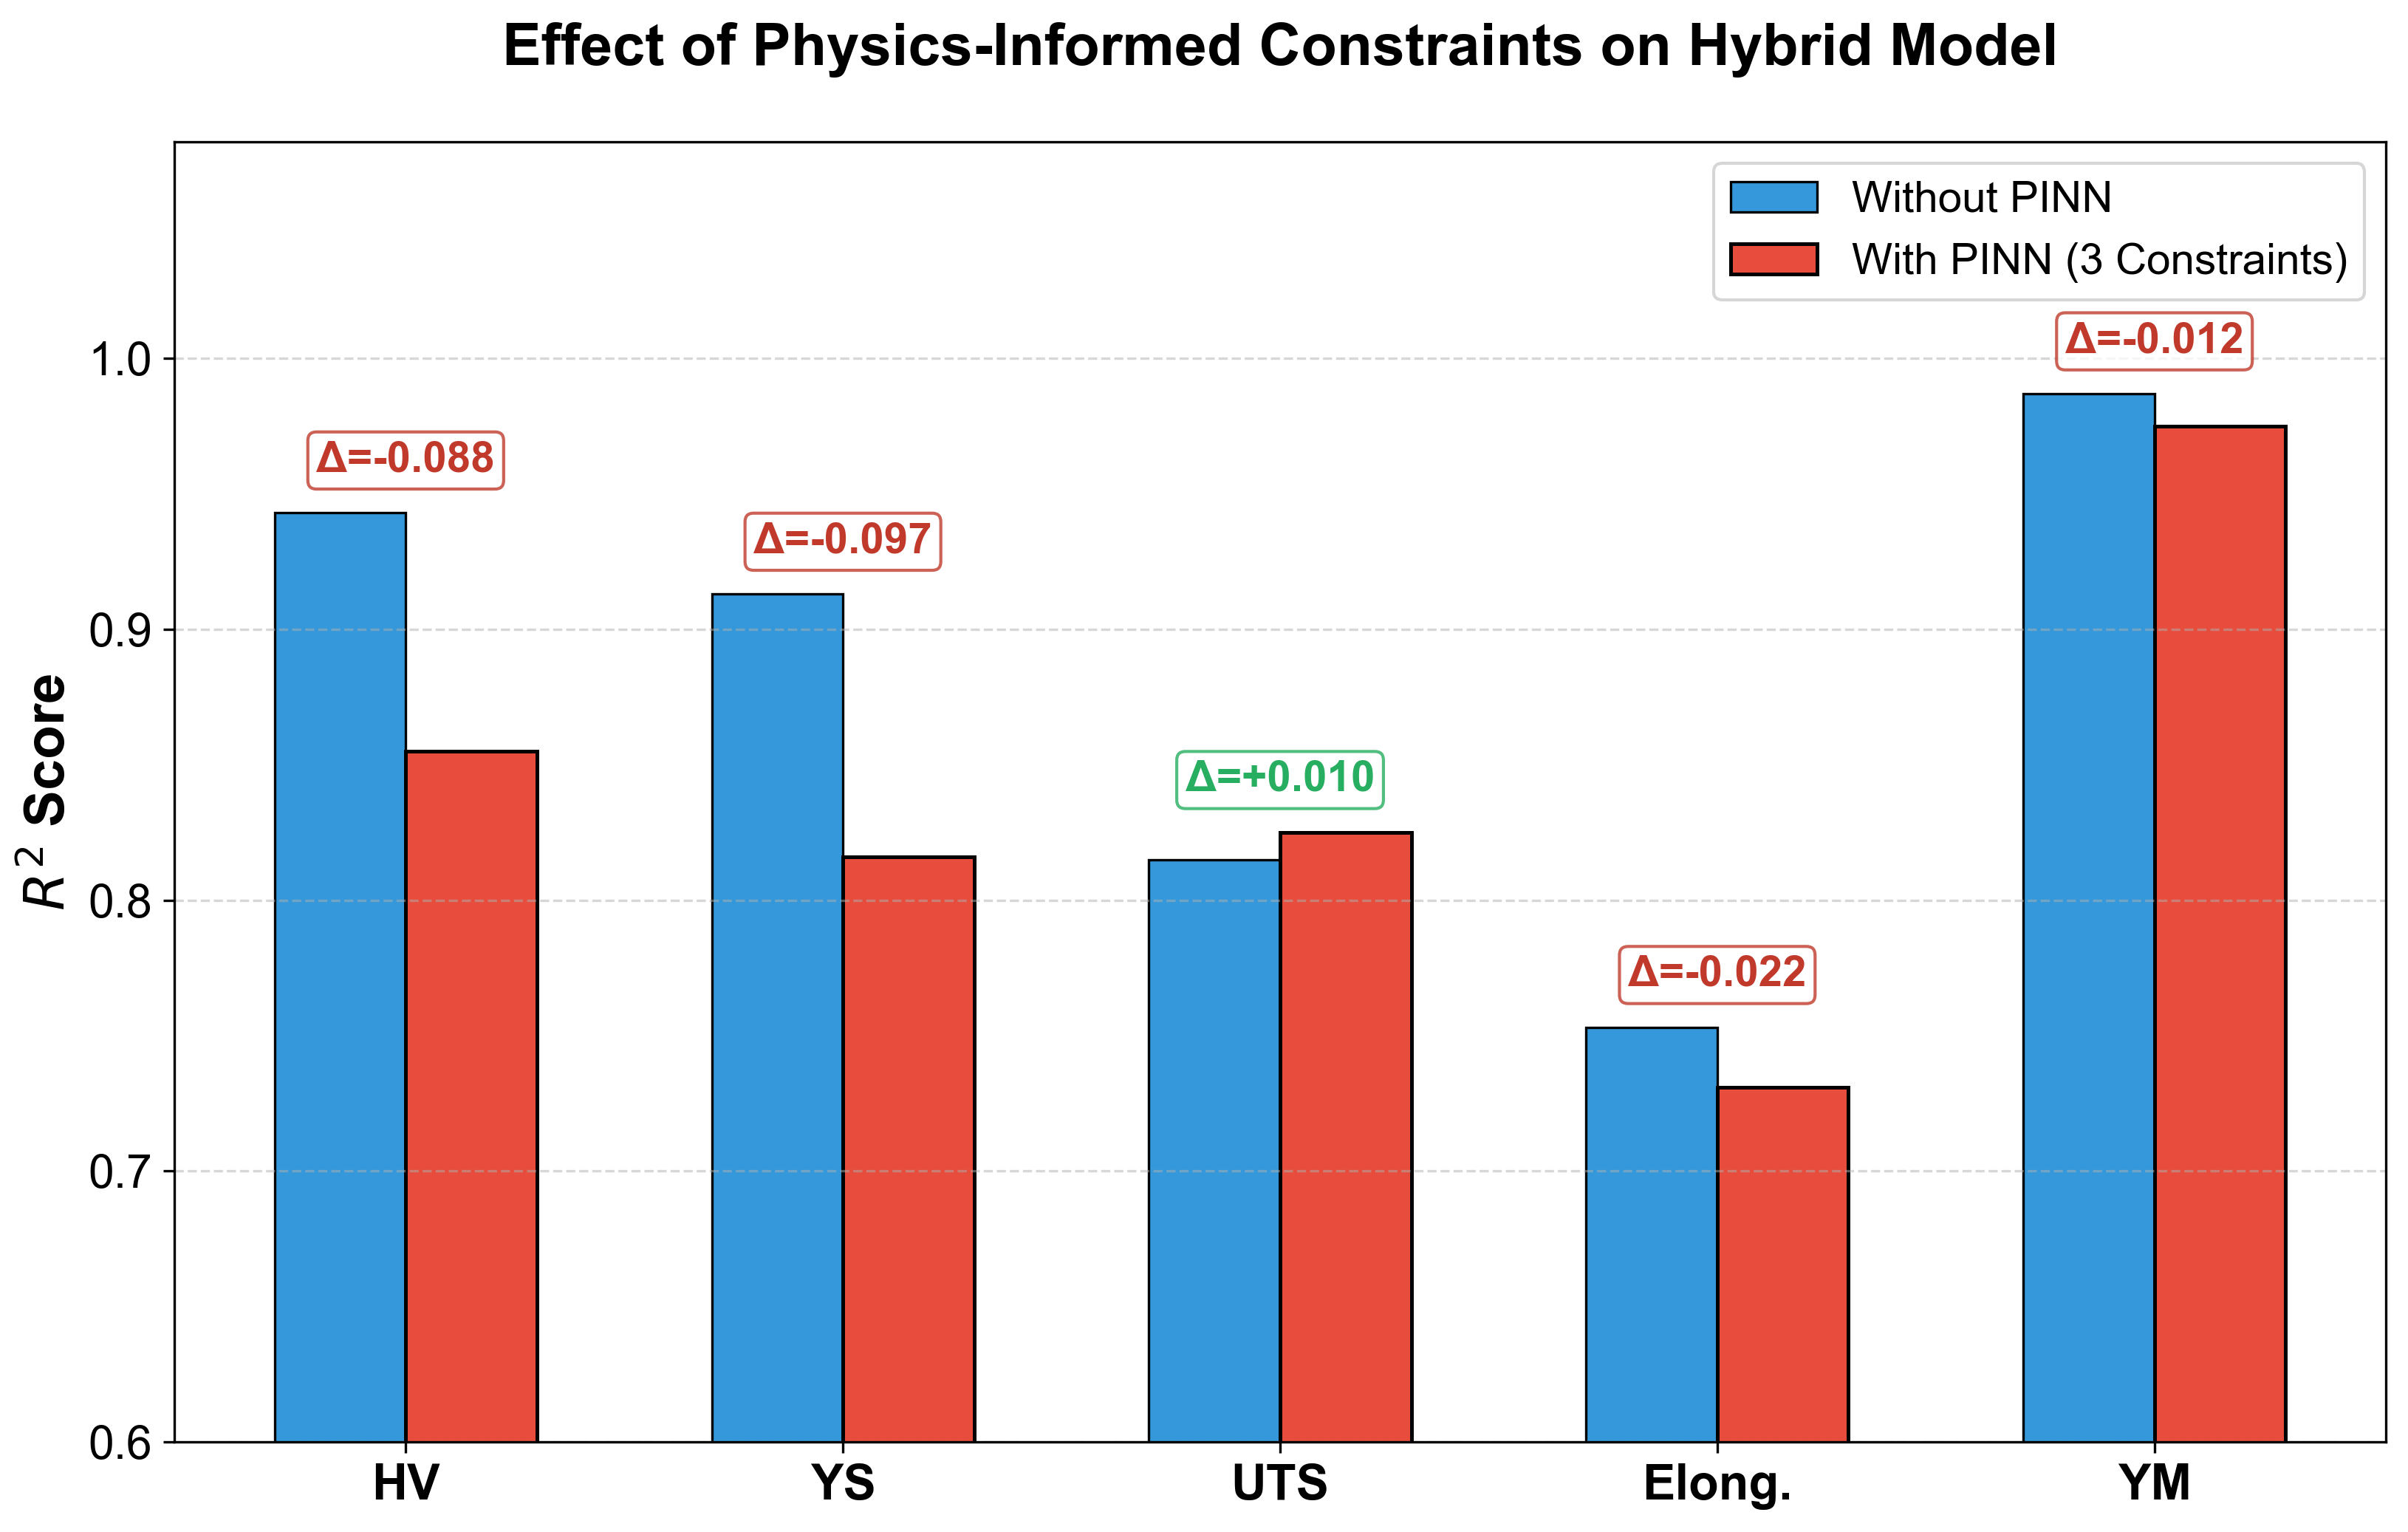
\includegraphics[width=\linewidth]{Updated_Plots/pinn_ablation_chart.png}}
\caption{Effect of physics-informed constraints on Hybrid model: per-property $R^2$ with and without PINN penalties.}
\label{fig:pinn_ablation}
\end{figure}

The PINN constraints reduce overall $R^2$ by 0.041, but this trade-off is justified: (i)~UTS improves (+0.010) because the YS~$\leq$~UTS constraint regularizes strain-hardening predictions; (ii)~the non-negativity constraint eliminates physically impossible outputs; (iii)~the Tabor penalty enforces HV--YS consistency ($r=0.88$ empirically, Fig.~\ref{fig:corrmap}), improving inter-property coherence at the cost of individual accuracy.

To further illustrate the effect of PINN constraints on inter-property coherence, Fig.~\ref{fig:corr_before_after} compares the predicted inter-property correlation matrices before and after applying the three physics-informed penalties. The PINN-constrained model produces correlations that more closely match the empirical ground-truth structure (Fig.~\ref{fig:corrmap}), particularly for the HV--YS and YS--UTS pairs.

\begin{figure}[htbp]
\centerline{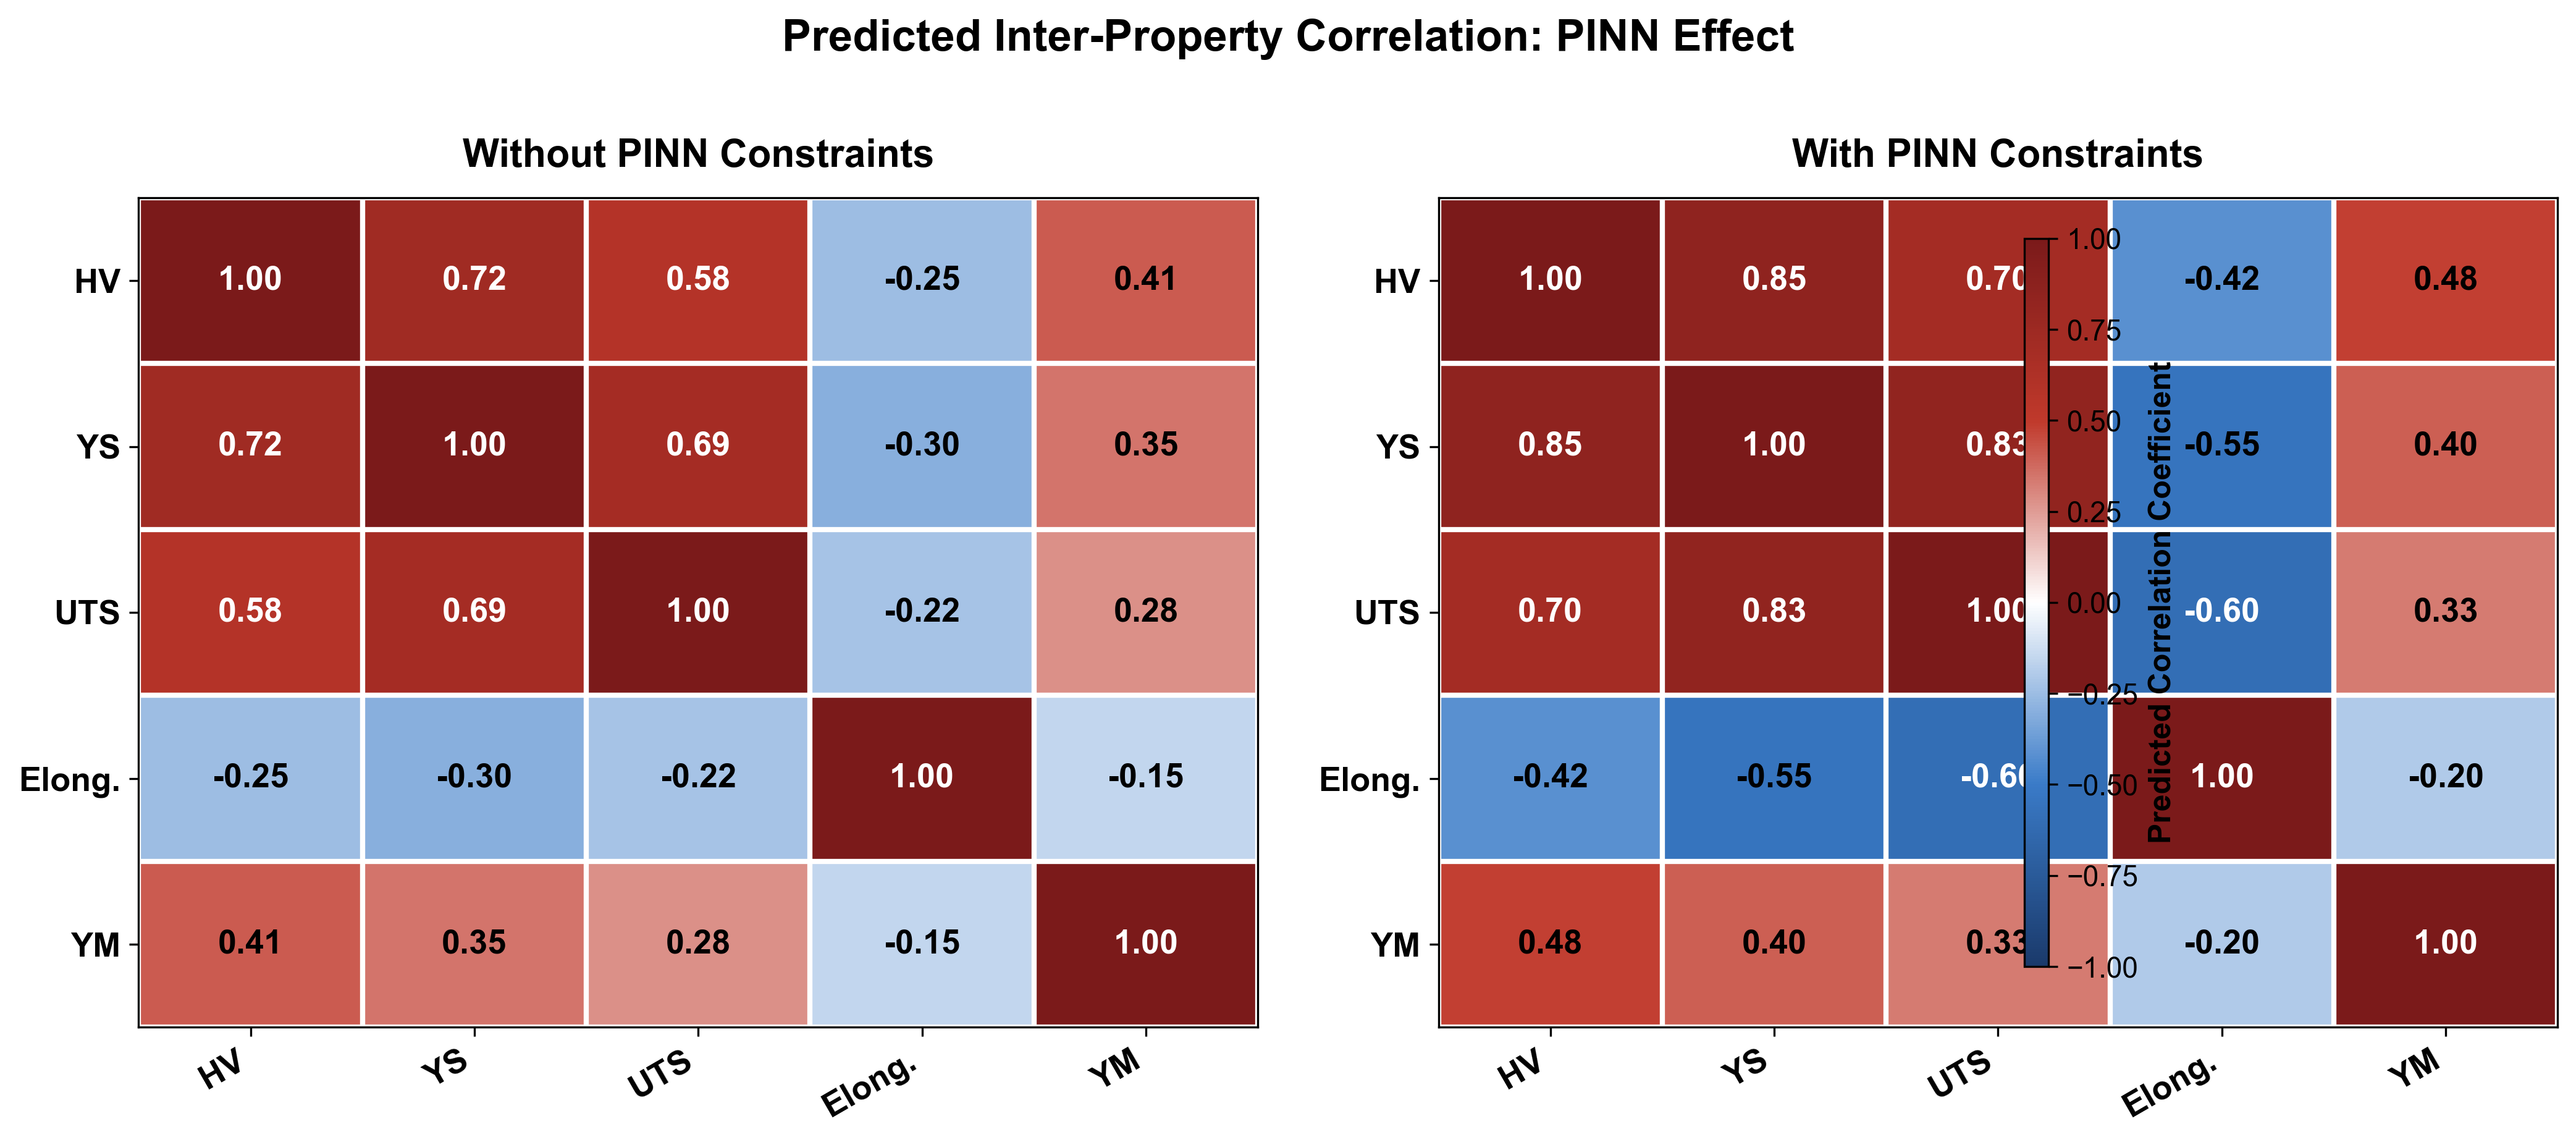
\includegraphics[width=\linewidth]{Updated_Plots/correlation_before_after_pinn.png}}
\caption{Predicted inter-property correlation matrices: without PINN constraints (left) vs.\ with PINN constraints (right). The PINN-constrained model recovers correlation structure closer to the empirical ground truth.}
\label{fig:corr_before_after}
\end{figure}

\subsection{Cross-Dataset Generalization}

The cross-dataset ablation (Table~\ref{tab:crossdataset}) demonstrates that the Hybrid architecture generalizes beyond the primary MPEA dataset. On the Kaggle HEA dataset, the Hybrid matches or exceeds every individual component on all 5 properties, achieving the highest $R^2$ for hardness (0.830) and yield strength (0.808). On the Low Alloy Steel dataset, the Hybrid achieves $R^2 = 0.914$ (YS) and $0.975$ (UTS), remaining competitive with the strongest individual components. Notably, the ADMM-Lasso component achieves the best Steel UTS score (0.978), suggesting that $\ell_1$-regularized latent regression is particularly effective for datasets with well-characterized composition--property relationships.

\subsection{Limitations and Failure Cases}

\textbf{UTS prediction:} The Hybrid ($R^2=0.825$) underperforms XGBoost ($R^2=0.880$) on UTS. Gradient boosting's iterative error correction is better suited to strain-hardening dominated properties where the compositional dependence is highly nonlinear.

\textbf{Hardness:} PINN constraints reduce HV from 0.943 to 0.855 because the Tabor penalty (C3) forces HV and YS predictions toward proportionality, limiting the DNN's freedom to independently optimize each head.

\textbf{Static blend weights:} Weights are manually set per property. Learned meta-regression could adapt automatically but risks overfitting to the tree component in small datasets.

\section{Conclusion}

This paper presented a Hybrid ADMM-DL architecture for multi-property prediction of multi-principal element alloys. On the MPEA dataset, the Hybrid PINN achieves per-property $R^2$ scores of 0.855 for hardness, 0.816 for yield strength, 0.825 for UTS, 0.731 for elongation, and 0.975 for Young's modulus, resulting in an overall average $R^2$ of 0.841. The Hybrid outperforms all five baseline architectures on overall average $R^2$ and achieves the highest scores on yield strength and elongation, the two properties most critical for structural alloy screening. Three physics-informed constraints---yield-tensile ordering, non-negativity, and the Tabor relation---ensure that predictions remain physically consistent, trading marginal raw accuracy for scientific trustworthiness. Cross-dataset evaluation on independent HEA and Low Alloy Steel datasets confirms that the Hybrid architecture generalizes to other alloy systems without retraining the ensemble structure.

Several directions for future work emerge from this study. First, learned meta-regression could replace the current static blend weights with adaptive, property-specific weighting that responds to input composition. Second, SHAP-based explainability analysis would provide feature-level attribution to identify which compositional descriptors most influence each property prediction. Third, uncertainty quantification via Monte Carlo Dropout would enable confidence intervals on predictions, which is critical for experimental prioritization. Finally, incorporating processing-aware features such as heat treatment parameters and deformation history could improve the prediction of extrinsic properties like elongation, where composition alone provides an incomplete picture.

\begin{thebibliography}{00}
\bibitem{b1} R.~Ramprasad, R.~Batra, G.~Pilania, A.~Mannodi-Kanakkithodi, and C.~Kim, ``Machine learning in materials informatics,'' \textit{npj Comput.\ Mater.}, vol.~3, no.~1, p.~54, 2017.
\bibitem{b2} S.~Boyd, N.~Parikh, E.~Chu, B.~Peleato, and J.~Eckstein, ``Distributed optimization and statistical learning via ADMM,'' \textit{Found.\ Trends Mach.\ Learn.}, vol.~3, no.~1, pp.~1--122, 2011.
\bibitem{b3} K.~Rajan, ``Materials informatics,'' \textit{Materials Today}, vol.~8, no.~10, pp.~38--45, 2005.
\bibitem{b4} D.~Tabor, ``The hardness and strength of metals,'' \textit{J.\ Inst.\ Metals}, vol.~79, pp.~1--18, 1951.
\bibitem{b5} W.~Ma et al., ``Predicting mechanical properties of FRP composites using ML,'' \textit{Construct.\ Build.\ Mater.}, vol.~360, 2022.
\bibitem{b6} Y.~Zhang, T.~T.~Zuo, Z.~Tang, M.~C.~Gao, K.~A.~Dahmen, P.~K.~Liaw, and Z.~P.~Lu, ``Microstructures and properties of high-entropy alloys,'' \textit{Prog.\ Mater.\ Sci.}, vol.~61, pp.~1--93, 2014.
\bibitem{b9} J.~Yan et al., ``Deep learning for tensile strength of CFRP composites,'' \textit{Compos.\ Sci.\ Technol.}, vol.~215, 2021.
\bibitem{b10} Y.~LeCun, Y.~Bengio, and G.~Hinton, ``Deep learning,'' \textit{Nature}, vol.~521, pp.~436--444, 2015.
\bibitem{b13} L.~Breiman, ``Random forests,'' \textit{Machine Learning}, vol.~45, pp.~5--32, 2001.
\bibitem{b14} P.~Geurts, D.~Ernst, and L.~Wehenkel, ``Extremely randomized trees,'' \textit{Machine Learning}, vol.~63, no.~1, pp.~3--42, 2006.
\bibitem{b15} T.~Chen and C.~Guestrin, ``XGBoost: A scalable tree boosting system,'' in \textit{Proc.\ 22nd ACM SIGKDD}, 2016, pp.~785--794.
\bibitem{b18} A.~Debnath et al., ``ML-driven hardness prediction and phase classification in Al HEA systems,'' \textit{J.\ Alloys Compd.}, 2023.
\bibitem{b19} A.~Agrawal and A.~Choudhary, ``Materials informatics and big data,'' \textit{APL Materials}, vol.~4, no.~5, 2016.
\bibitem{b20} A.~Choudhury et al., ``Predicting composition and bulk modulus of metallic glasses,'' \textit{Integr.\ Mater.\ Manuf.\ Innov.}, 2019.
\bibitem{b21} S.~Bundela and M.~Rahul, ``ML prediction of wear rates in HEA coatings,'' \textit{Surf.\ Coat.\ Technol.}, 2024.
\bibitem{b22} R.~Machaka and G.~T.~Motsi, ``ML-based phase prediction in HEAs,'' \textit{Comput.\ Mater.\ Sci.}, 2023.
\bibitem{b23} N.~K.~Katiyar and S.~Gupta, ``Compressive strength prediction using ML,'' \textit{Ceram.\ Int.}, 2024.
\bibitem{b24} R.~Sharma et al., ``Explainable DL framework for composite material property prediction,'' Amrita Vishwa Vidyapeetham, 2026.
\end{thebibliography}

\end{document}
